\chapter{A Review of Home-brewing and User Experience through Performance} \label{l-r}

\section{Introduction} \label{l-r--introduction}

This first section (\ref{l-r--home-brewing}) of this chapter discusses the current landscape for home-brewing and it's integration with technology. The following section (\ref{l-r--user-experience-performance}) explores the relationship between performance, user experience and modern web development. The analysis and design phase of this project will consider these topics. Finally, section \ref{l-r--summary} summarises the chapter.

\section{Home-brewing} \label{l-r--home-brewing}

Last year, BBPA (The British Beer and Pub Association) estimated pubs in the UK had ``fallen by 19\% since 2000: from 60,800 to 49,433 in 2012". \cite{BBPA}

Craft and independent brewing is on the up however. SIBA (The Society of Independent Brewers), saw an increase of  SIBA’s membership has grown by 49 members in 2015. \cite{SIBA}

Home-brewing, brewing beer on a small personal scale, has been around for thousands of years and has grown popular in the last few years.

\subsection{Overview of a home-brew}

\cite{brewing_overview} suggest there are four main ingredient and four main steps to brewing beer.

The four main ingredients of a brew are: \textbf{Malt}, \textbf{Hops}, \textbf{Yeast} and \textbf{Water}.

\begin{itemize}
  \item \textbf{Malt} is a grain used to create the sugar for the yeast and determines how strong a beer is.
  \item \textbf{Hops} determines how bitter or sweet a beer is as well as other flavours and aromas.
  \item \textbf{Yeast} consume the sugars from the malt and convert them to alcohol and carbon dioxide (fizz). The yeast converts the wort (unfermented beer) becomes beer.
  \item \textbf{Water} most of a brew is water, up to 90\% by volume.
\end{itemize}

Taking these ingredients there are four steps to take: \textbf{Malting}, \textbf{Mashing}, \textbf{Boiling (and Cooling)} and \textbf{Fermenting (and Conditioning)}.

\begin{enumerate}
  \item \textbf{Malting} starts the process of converting the ingredients into beer. This process results in dried grains by heating (or kilning).
  \item \textbf{Mashing} soaks the malted grains for the previous step in hot water, this produces the maltose to feed the yeast. This produces wort for the next step.
  \item \textbf{Boiling (and Cooling)} the wort santises the brew, it's at this point the hops are added. After cooling the yeast is then added.
  \item \textbf{Fermenting (and Conditioning)} starts to occur, this can last from weeks to months depending on the strength.   Once this step is complete it's time to bottle the brew.
\end{enumerate}

From the above process it is clear that this process is not trivial.

\subsection{A comparison of home-brewing and OSS} \label{l-r--compare-home-brewing-and-oss}

Sharing recipes, set-ups and brewing techniques is analogous to the open source communities surround software and hardware. Bringing the two together is mutually beneficial.

With the popularity of affordable and accessible computing with platforms such as Raspberry PI and Arduino, introducing computing technologies into home brewing means more automation and control.

Due to the open source nature of these platforms, many systems have been created. One example is BrewPi, a fermentation temperature controller for brewing beer or wine. \cite{brewpi}

This merge of physical creating and software can be seen all across the tech community. One great example is in farming with the MIT Open Agriculture Initiative, ``Every time users grow and harvest, they will contribute to a library of climate recipes that can be borrowed and scaled so that users around the world can gain access to the best and freshest foods.". \cite{climate_recipes}

Ultimately, the Internet is the perfect platform for this type of recipe sharing and collaboration.

\subsection{Existing home-brewing solutions and APIs} \label{l-r--exisiting-home-brewing-solutions}

Data formats have been created to handle brewing recipes and other brewing data, the most mature and popular of which is BeerXML. BeerXML uses the XML format for brewing data. \cite{beerxml} Open and standardized formats in general mean better portability, compatibility for data.

With a decline in usage of XML \cite{jsonxml}, a JSON alternative has been created aptly named BeerJSON. \cite{beerjson}

Malt.io is a community website for these brewing recipes. With the options for revision history and `cloning' of recipes it is clear it is inspired by the popular Git repository and social coding network GitHub. \cite{malt.io}

There are many software solutions for various parts of the brewing process. Some of which are reviewed in section \ref{a-d--review-of-existing-software}.

\section{User Experience through Performance} \label{l-r--user-experience-performance}

User experience (referred to as UX), is how a user feels while using a system. There are many aspects to user experience such as usability and accessibility. \cite{what_is_ux}

One of the most important aspects of user experience is the performance. When looking at the web specifically, performance in essence is the perceived speed of websites and the actions taken on them.

When designing and building on the web, performance should be considered at the same level as aesthetics. \cite{performance_is_ux}

\subsection{Speed and Timing} \label{l-r--speed}

There is a lot of research into users' relationship with time.

\cite{usability_engineering} shows time affect how users behave towards a system. A system feels instantaneous with actions taken under 0.1 seconds. Anything over 1 second a user can lose their flow of though on an action. After 10 seconds a users will lose attention and start to multi-task.

In terms of relative time, users percieve faster or slower tasks when there is a difference of 20\% in time. \cite{setting_a_performance_budget}

Google have ``always viewed slain peed as a competitive advantage", when running experiments by introducing artificial delays into searches ``slowing down the search results page by 100 to 400 milliseconds has a measurable impact on the number of searches per user of -0.2\% to -0.6\%". \cite{speed_matters}

Performance delays aren't merely an annoyance, a bad first impression can result in users not returning. \cite{why_web_performance_matters} confirm that ``88\% of online consumers are less likely to return to a site after a bad experience". Delays are stressful. As shown by figure \ref{figure-stress-mobile-delay}, \cite{ericsson} found that mobile delays are more stressful than standing in line at a shop or even watching a horror movie.

\begin{figure}[H]
  \centering
    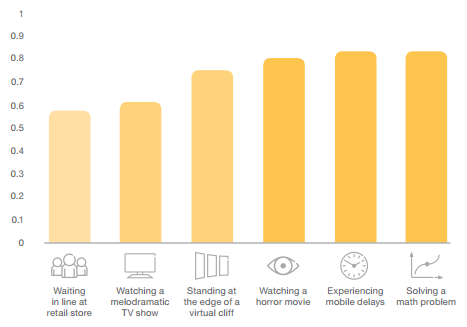
\includegraphics[width=\textwidth,height=\textheight,keepaspectratio]{stress_mobile_delay}
  \caption{Cognitive load associated with stressful situations \protect\cite{ericsson}}
  \label{figure-stress-mobile-delay}
\end{figure}

There is a clear demand for performance when looking at the topic of blocking web advertising. A controversial topic as of writing, one of the benefits shown is the increase in performance for users especially on mobile platforms. Typically a browser extension would be used to block adverts. Brave, a browser built with advertisement blocking in from the start claims on page load 60\% of the time is being caused by advertisement resources. \cite{brave}

\subsection{Perceived Performance} \label{l-r--perceived-performance}

Before discussing achieving good performance through development aspects, it's worth noting a user is only perceiving this performance. If this perceived performance often can be achieved without technical development.

Optimistic user interfaces (UIs) show a user feedback before the corresponding action has taken place thus giving an excellent perceived performance.

An example of this is the Instagram like button. On press of the like button the application doesn't wait for a round trip to the server to check that action was carried out successfully, instead it shows the user that they have liked the post immediately with the `optimism' that the action will be carried out. \cite{performing_actions_optimisitically}

Lazy-loading is the method of loading content (often images) after initial load for performance. This is often used as part of an optimistic UI.

Using images as an example, figure \ref{figure-lazy-loading-images} shows the generation of a placeholder based the source image for a smoother smoother transition. One technique to achieve this is to create a tiny thumbnail, let the browser resize and then blur to create a gradient based on the image's colour palette. \cite{image_colours_lazy_loading}

\begin{figure}[H]
  \centering
    
\includegraphics[width=\textwidth,height=\textheight,keepaspectratio]{lazy_loading_images}
  \caption{Example of placeholder when lazy loading \protect\cite{image_colours_lazy_loading}}
  \label{figure-lazy-loading-images}
\end{figure}

\subsection{Measuring and techniques} \label{l-r--measuring-and-techniques}

Measuring performance is important, data metrics allows for better. Tools such as Google's PageSpeed and WebPageTest give developers metrics across all aspects of web performance.

One metric is SpeedIndex ``is the average time at which visible parts of the page are displayed". The benefit to this metric is it helps measure a usable website over just a loaded website. A website may be usable without all of the content having loaded in. \cite{speed_index}

Best practices include optimising a website's resources and where they are retrieved from. With CSS file growing larger in size a emerging approach is through Critical CSS. Serving a part of the CSS on load, loading the rest asynchronously and then caching it all for further visits. \cite{fast_as_heck}

\subsubsection{Performance Budgets} \label{l-r--performance-budgets}

Just like budgeting finances, having a performance budget can give a starting point for working with performance in mind. Having this initial constraint can ensure that performance will be thought of while designing. \cite{performance_budget}

One way to find initial metrics is off of similar websites. As described in section \ref{l-r--speed}, setting the target for the metrics at 20\% will mean users perceive the site as faster.

\subsubsection{Front-end Frameworks and Libraries} \label{l-r--frameworks}

Frameworks and libraries can improve development of websites but it is important to consider file size and overall performance of JavaScript when looking at performance.

Frameworks are generally expensive for any mobile devices, also there is a loss of control as to what final code is produced. \cite{cost_of_frameworks}

\begin{figure}[H]
  \centering
    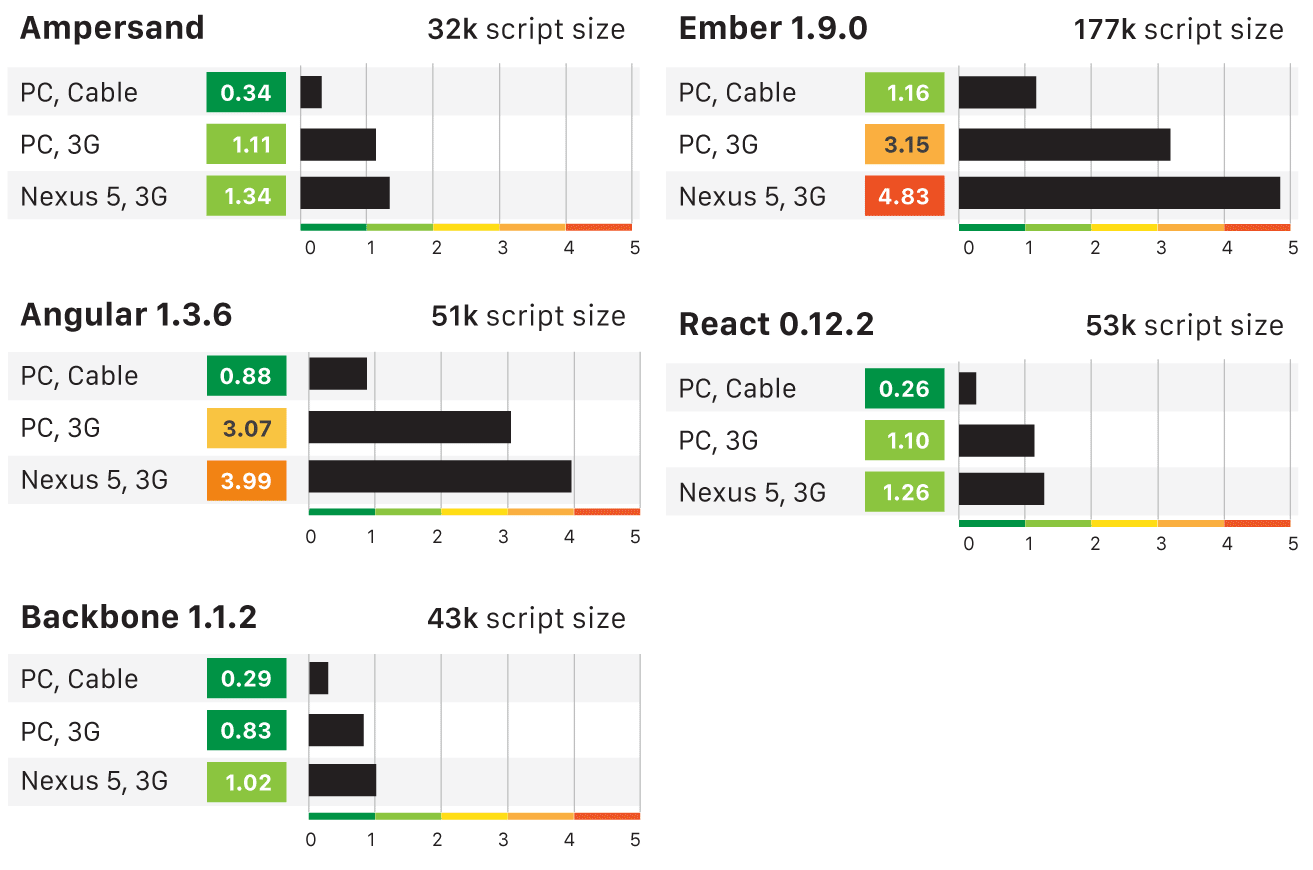
\includegraphics[width=\textwidth,height=\textheight,keepaspectratio]{mvc_performance}
  \caption{Average first render times (seconds) \protect\cite{performance_mvc}}
  \label{figure-average-first-render}
\end{figure}

Figure \ref{figure-average-first-render} shows React has the quickest render on PC, with a cable network connection. Lightweight libraries like Backbone and Ampersand are also comparable to React's performance. Angular with a smaller size and  having much features performs much slower overall. Ember also with more features than React is both larger in file size and slower overall.

\subsubsection{Animation} \label{l-r--animation}

60 frames per second is the goal to hit when animating on the web due to most screens refreshing at this rate, if a site drops below this there is the screen judders commonly known as `jank'. \cite{jank}

When animating with CSS generally the properties to stick to are \verb|transform| and \verb|opacity|. These properties are hardware accelerated and therefore reduce jank. \ref{high_performance_animations} \ref{css_triggers}

Using the \verb|will-change| property tells the browser there is a plan for it to animate. This is to replace using \verb|translateZ()| as a hack to force the browser to hardware accelerate. \ref{animations_and_performance}

Interestingly, Microsoft Edge do not plan to implement \verb|will-change| as they claim it is already optimised. \cite{will_change_edge}

There are attempts to formalise these animation techniques into projects such as RAIL and LIP. \cite{introducing_RAIL} \cite{FLIP}

\subsection{Web typography} \label{l-r--web-type}

Good typography is a great way to improve user experience through usability and accessibility. For example, for some dyslexic users can find incorrectly spaced text hard to read through something called `rivers'. \cite{dyslexia}

Due to the popularity of web fonts it's easy to think this is a quick and easy way to improving the typographical user experience of your website. However, just using a web font alone doesn't guarantee a better typography for users. Web fonts are slow, and if poorly implemented can leave users with no content at all on bad connections. This can create something called the Flash of Invisible Text (or `FOIT') where the browser hides web font text until the web font has fully loaded. \cite{FOIT}

A great reading experience with default system typefaces is easily achieved. As \cite{against_webfonts} explains: ``Typography is not about aesthetics, it's about serving the text. If even a small percentage of people don't consume your content due to a use of web fonts, your typography is failing."

There are ways to avoid FOIT through progressively applying fonts once they're loaded. These approaches work well for repeat visits to a website as these fonts can then be cached. \cite{FOIT}

\subsection{Progressive Enhancement} \label{l-r--progressive-enhancement}

Progressive enhancement is treating extra layers of enhancement (such as images, dynamic behaviours) is optional. With this attitude HTML is the only thing that should be relied upon. Sometimes even HTML can't reach the user (something discussed in section \ref{l-r--offline-first}). \ref{progressive_enhancement}

There are arguments against progressive enhancement and that it can't always be achieved. There is a lot of discussion towards the progressive enhancement of JavaScript specifically. \ref{progressive_enhancement_dead} claims that JavaScript can be assumed to be part of the web platform.

\subsection{Offline First} \label{l-r--offline-first}

``Frequently not having any data connection in even the wealthiest and most developed cities of the world has led us to conclude that no, the mobile connectivity/bandwidth issue isn’t just going to solve itself on a global level anywhere in the near future." \cite{hello_to_offline_first}

One of the biggest problems connecting to the Internet across the world is not the availability of devices but the network connections. Every year global mobile broadband subscriptions increases by 25\%. In Q4 2015 there were 21 million in India, 21 million in Africa, 20 million APAC (excluding China and India). By comparison, 5 million Europe and 5 million in North America. \cite{ericsson}

India's biggest e-commerce site Flipkart found 63\% users reaching their mobile site via a 2G network. \cite{flipkart} Developing with a stable and fast network connection in mind is not an option if considering these users.

A offline experience can be progressively enhanced with cached content managed by a Service Worked but even the poorest connection is online. Described by Jake Archibald: ``Lie-Fi is like offline, but it trolls you by pretending to be online. It'll attempt to make a connection for minutes and still fail." \cite{supercharging_page_load}

This uncertainty with network connectivity means an site can never assume a user is completely offline.

Previous methods of caching content was through using Appcache, however the lack of control made it a very dangerous technology to use. \cite{appcache}

\subsection{Workers} \label{l-r--workers}

When developing on the web historically this meant running client-side Javascript in a single threaded environment. With the introduction of Workers web content can be handled with background tasks.

The two main Workers are Service Workers and Web Workers.

Web Workers create background tasks that can run Javascript that interface back and forth between the main JavaScript tasks. A use case of Web Workers is syncing data between a clientside database and a remote database. \cite{using_web_workers}

Service Workers can be seen more as a proxy server between your server and your main JavaScript thread, the key concept is that of `installing' a Service Worker file to the browser itself registered to a origin. Service Workers are asynchronous and so don't have access to APIs such as XHR.

Some use cases of Service Workers include, caching for a better (and sometimes offline) experience, Push notifications, background data syncing. \cite{service_worker}

\subsection{Performance based projects}

Google have set-up the Accelerated Mobile Pages (AMP) Project as a way to create content optimized for mobile. This project grew from a discussion ``between publishers and technology companies about the need to improve the entire mobile content ecosystem for everyone". AMP is constrained to ensure reliable performance, at the cost of limited flexibility in content. \cite{intro_to_amp}

\section{Summary} \label{l-r--summary}

In Chapter 1 we proposed user through performance with the example of home-brewing.

In this chapter home-brewing was introduced (section \ref{l-r--home-brewing}) followed by an extensive review of user experience through performance (section \ref{l-r--user-experience-performance}).

The next chapter presents the design of a progressive home-brewing based web application following the discussion from this chapter.
